\section{Sistemas Eletrônicos}
Texto a ser redigido.

\subsection{Raspberry Pi 3 Model B Plus}

A Raspberry Pi é um microcomputador sistema operacional Linux, que foi escolhida para ter o programa embarcado que controla e monitoriza a estufa devido a facilidade de acesso aos seus pinos GPIO para conectar diversos sensores e atuadores, como ela já tem conectividade Wi-Fi, será facilmente facilmente conectada a internet apenas acessando a rede local do usuário e ela já tem autorização pela Anatel, com suas entradas USB, é possível conectar uma câmera USB e utilizá-la para monitorizar a estufa. [RASPBERRY PI FOUNDATION, 2018]

Especificações:

\begin{itemize}
	\item Raspberry Pi 3 Model B Anatel
	\item Processador Broadcom BCM2837 64bit ARMv8 Cortex-A53 Quad-Core
	\item Clock 1.2 GHz
	\item Memória RAM: 1GB
	\item Adaptador Wifi 802.11n integrado
	\item Bluetooth 4.1 BLE integrado
	\item Conector de vídeo HDMI
	\item 4 portas USB 2.0
	\item Conector Ethernet
	\item Interface para câmera (CSI)
	\item Interface para display (DSI)
	\item Slot para cartão microSD
	\item Conector de áudio e vídeo
	\item GPIO de 40 pinos
	\item Número de homologação Anatel: 04908-17-10629 
	\item Dimensões: 85 x 56 x 17mm[1]
\end{itemize}

\subsection{Sensor de nível de água eletrônico - ON/OFF - US23}

Este sensor de nível é uma chave ON/OFF (Liga/desliga) que muda o estado de aberto para fechado quando a água atinge certo nível e abre quando o nível da água fica abaixo de outro determinado nível. Este sensor pode chavear diretamente cargas de até 10W 220V, como bobinas de contatores ou pequenas lâmpadas de sinalização. No caso do projeto da estufa, ele irá chavear uma tensão de 3.3 V e corrente de 3.3 mA, garantida por um resistor de 10K$\Omega$. 

E serão utilizadas duas boias na seguinte disposição da figura 1. [EICOS SENSORES, 2018]

\begin{figure}[H]
	\centering
	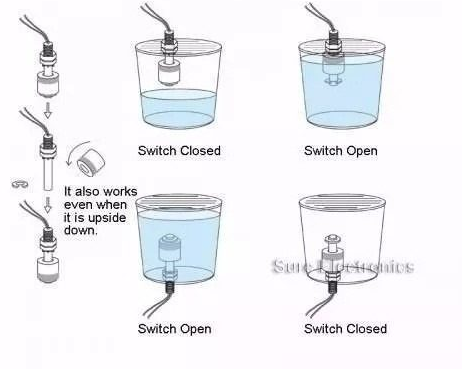
\includegraphics[width=10cm]{figuras/eletronica_1.png}
	\caption{Disposição das Boias no Reservatório} \label{eletronica_1}
\end{figure}

Uma ao fundo para definir se o nível da água está baixo e um em cima definir o nível de água baixo.  A leitura do estado dos sensores será feita através do pino GPIO, onde o estado HIGH (tensão de 3.3V ) indica que o sensor foi ativado e o estado LOW(tensão de 0V) indica que ele está desativado. [EICOS SENSORES, 2018]

Este sensor de nível utiliza um sensor magnético e não mercúrio que seria prejudicial à saúde.[EICOS SENSORES, 2018]

Características:

\begin{itemize}
	\item Raspberry Pi 3 Model B Anatel
	\item Comprimento do cabo: 36cm
	\item Máxima potência da carga: 10W
	\item Máxima tensão: 220V DC
	\item Máxima corrente de chaveamento: 0.5A
	\item Máxima corrente de carga: 1A
	\item Resistência do contato: 0.1 $\Omega$
	\item Temperatura de trabalho: -10°C ~ + 60°C
	\item Dimensões da boia: 23mm x 22mm
	\item Comprimento do sensor: 57mm
	\item Diâmetro do eixo: 8mm
	\item Diâmetro da rosca: 9mm
\end{itemize}

\subsection{Optoacoplador 4N25}

São dispositivos de proteção em circuitos eletrônicos que precisam trabalhar com diferentes tensões. No projeto da estufa eles serão utilizados para conectar a Raspberry a dispositivos que trabalham com tensão diferente de 3.3V, que é a tensão dos pinos GPIO, e para evitar uma sobrecarga de corrente nela.  [VISHAY SEMICONDUCTORS]

O optoacoplador escolhido foi 4N25, que é constituído por um diodo emissor de luz e um foto transistor bipolar. E funciona como mostrado na figura abaixo:

\begin{figure}[H]
	\centering
	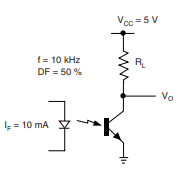
\includegraphics[width=5cm]{figuras/optocoaplador.png}
	\caption{Funcionamento do optoacoplador} \label{optocoaplador}
\end{figure}

A Raspberry irá controlar o LED interno do optoacoplador, quando o LED está aceso o transitor é “ativado” e permite a passagem de corrente através dele. E quando o LED está apagado o trasnsitor fica em situação de corte e não permite a passagem de corrente.
Para o projeto da estufa foi confeccionada uma placa com com 8 optoacopladores, figura 3,  que serão conectados aos relés que garantirão uma proteção a mais para o circuito. [VISHAY SEMICONDUCTORS]

\begin{figure}[H]
	\centering
	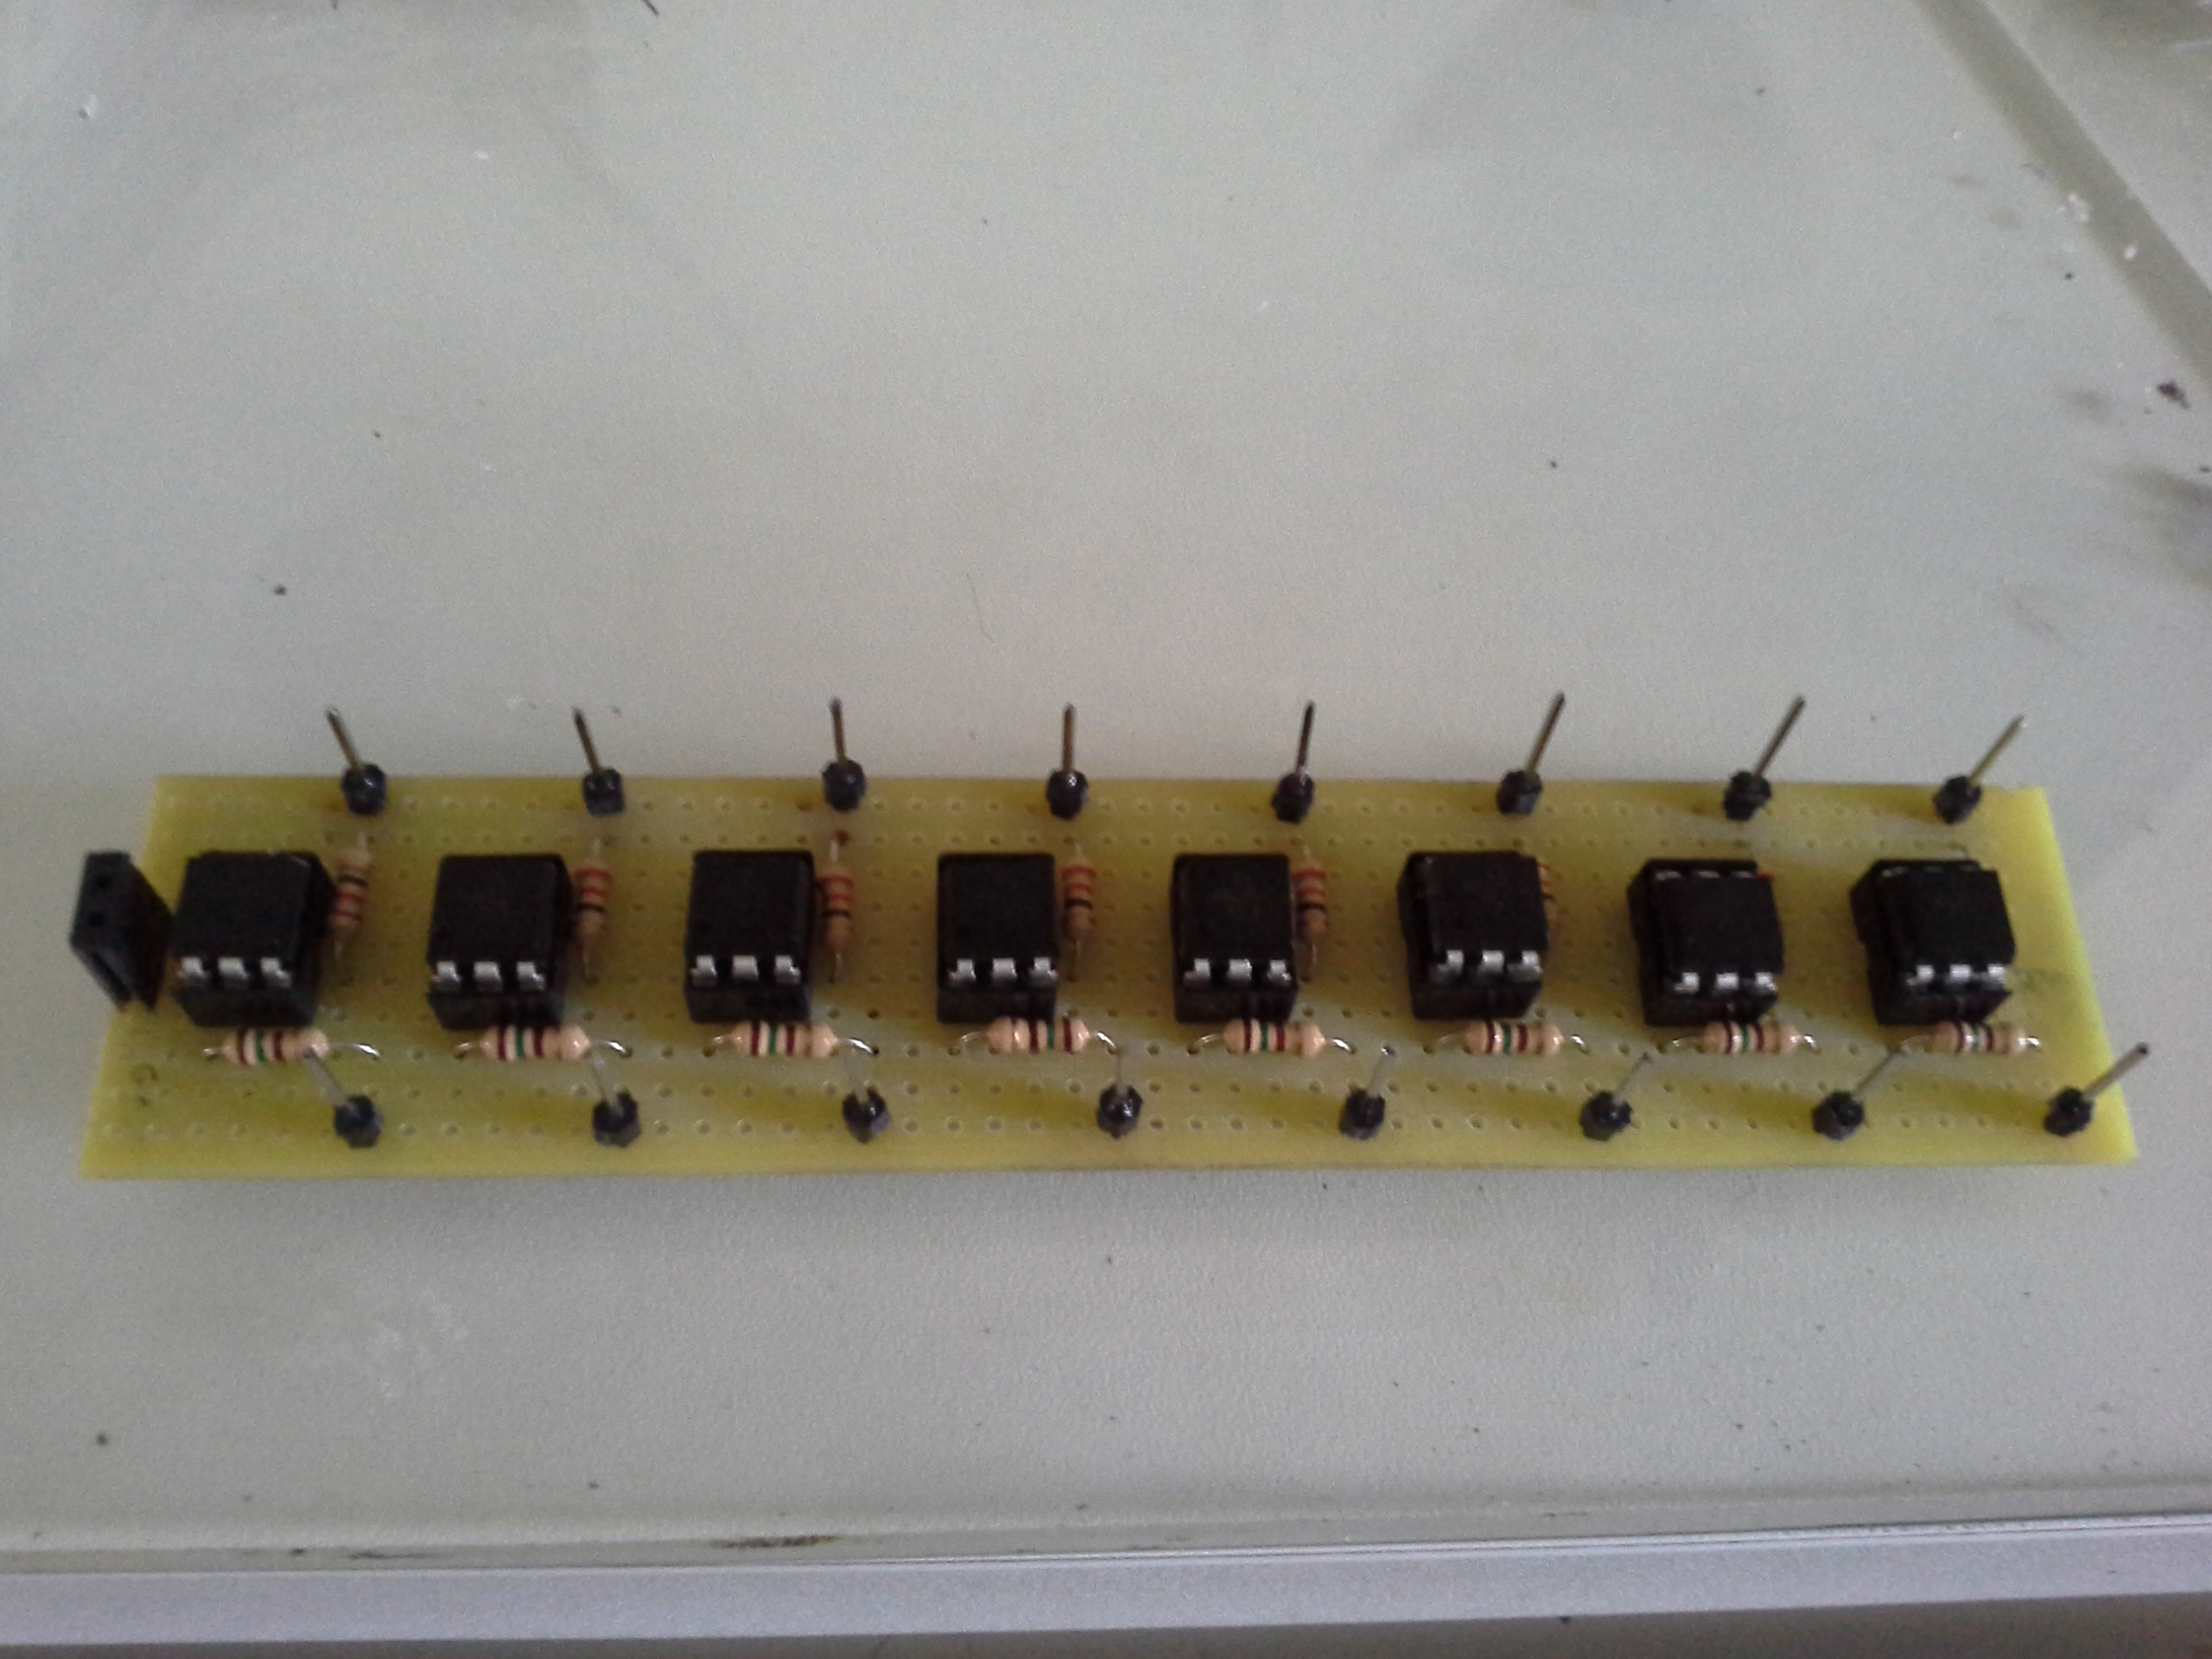
\includegraphics[width=15cm]{figuras/optoacopladores.jpg}
	\caption{Optoacopladores} \label{optoacopladores}
\end{figure}

\subsection{Relé}
Os relés basicamente são dispositivos elétricos que tem como função produzir modificações súbitas, porém predeterminadas em um ou mais circuitos elétricos de saída. O relé tem um circuito de comando, que no momento em que é alimentado por uma corrente, aciona um eletroímã que faz a mudança de posição de outro par de contatores, que estão ligados a um circuito ou comando secundário. Resumidamente podemos dizer que todo relé se configura como um contato que abre e fecha de acordo com algum determinado fator ou configuração. Alguns relés são bem pequenos e fáceis de serem manipulados, testados e trocados, justamente por existir vários tipos de construções mecânicas para relés. [Braga, 2012]

O relé é um componente eletromecânico, ou seja, ele conta com uma parte mecânica de contato e o acionamento ocorre através da corrente elétrica em uma bobina. Na imagem abaixo é possível visualizar todos os componentes de um relé eletromecânico. [Braga, 2012]

\begin{figure}[H]
	\centering
	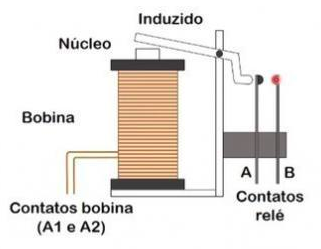
\includegraphics[width=5cm]{figuras/rele.png}
	\caption{Relé Internamente} \label{rele}
\end{figure}

No projeto da estufa os relé serão utilizados para acionar as 3 bombas de aágua responsáveis pela circulação de água, os coolers de circulação de ar, as válvulas solenóides que controlam a torca de água do reservatório, as lâmpadas da estufa e o compressor de ar do reservatório de água.
Como serão vários dispositivos e consequentemente vários relés, o grupo optou por comprar um módulo relé de 8 canais.[Braga, 2012]

Ele será ativado pelo pinos GPIO da Raspberry Pi, que estarão isolados por um optoacoplador.


\subsection{Conversor Analógico para Digital}

A Raspberry Pi não possui conversor AD integrado, como alguns microcontroladores, e alguns dos sensores utilizados no projeto precisam de um, pois apresentão seus dados de forma analógica. Para contornar essa dificuldade haviam duas possibilidades, utilizar um microcontrolador com conversor analógico integrado e realizar a comunicação do mesmo com a Raspberry, ou conectar um conversor AD diretamente a Raspberry. A opção escolhida pelo grupo foi a segunda, pelo baixo custo e pela oportunidade de aprender a utilizar um conversor AD pelos membros do grupo de eletrônica.[NXP, 2013]

O conversor escolhido foi PCF8591, que é um dispositivo de aquisição de dados CMOS de 8 bits de alimentação única e baixo consumo de energia, com quatro entradas analógicas, uma saída analógica e uma interface de barramento I2C serial. Três pinos de endereço A0, A1 e A2 são usados para programar o endereço de hardware, permitindo o uso de até oito dispositivos conectados ao barramento I2C sem hardware adicional. O endereço, o controle e os dados do dispositivo são transferidos serialmente por meio do barramento I2C bidirecional de duas linhas.[NXP, 2013]

As funções do dispositivo incluem multiplexação de entrada analógica, função de faixa e retenção no chip, conversão de analógico para digital de 8 bits e conversão de digital para analógico de 8 bits. A taxa de conversão máxima é dada pela velocidade máxima do barramento I2C.[NXP, 2013]

O esquemático do circuito do conversor AD se encontra na figura abaixo:

\begin{figure}[H]
	\centering
	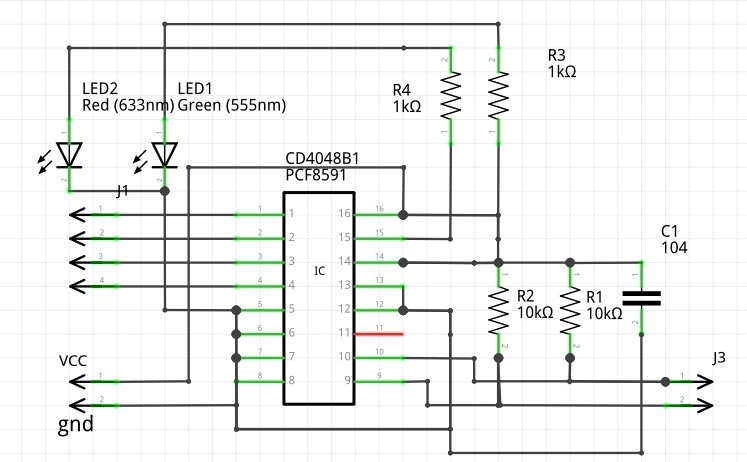
\includegraphics[width=12cm]{figuras/circuito_1.png}
	\caption{Circuito PCF8591} \label{circuito_1}
\end{figure}

Para realizar a leitura dos dados obtidos nas suas entradas analógicas foi nessesário importar a biblioteca smbus.[NXP, 2013]

Para testar seus funcionamento foi utilizado um potenciômetro de 10K$\Omega$, que variava a tensão de entrada no pino A0 do conversor entre 0V e 5V. O resultado obtido foi satisfatório com precisão de 0.01 V.


\subsection{Sensor LDR}

LDR (Light Dependent Resistor), ou fotoresistror, é um dispositivo resistivo que tem a sua resistência alterada de acordo com a quantidade de luz que atinge seus terminais. O componente é feito de um semicondutor de resistência elevada. O sensor apresenta uma alta sensibilidade, com uma resposta rápida as variações de luz e é sensível a todo o espectro visível de luz.[1]

\subsubsection{Características elétricas}

O LDR apresenta em uma temperatura ambiente uma variação de resistência de aproximadamente 8$\Omega$ até 20K$\Omega$, no escuro total a resistência atinge um valor elevado e 1M$\Omega$. O seu pico de resposta é com o comprimento de onda de 540nm, podendo funcionar dentro de um ambiente com temperaturas variando de -30℃ até 70℃.[Jawaaz Ahmad, 2016]

O sensor aguenta nos seus terminais uma diferença de potencial de até 150 Volts. A leitura do sensor é feita através de um divisor de tensão que é causada pela variação da resistência devido a diferença de iluminação. A tensão lida na saída do divisor de tensão é lida por um conversor AD e assim é transformada em dados para o microcontrolador.[Jawaaz Ahmad, 2016]

\subsubsection{Princípios físicos de funcionamento}

Um LDR trabalha com a fotocondutividade, que é um efeito ótico onde a condutividade de um material aumenta com a absorção de luz do semicondutor. A exposição à luz do sensor faz com que fótons dessa fonte de luz ao caírem no sensor excitem os elétrons da camada de valência do semicondutor que compõem o sensor. Os elétrons são excitados até adquirirem energia suficiente para chegar a camada de condução do material. Quanto mais elétrons são excitados até a camada de condução do semicondutor, mais corrente passa a fluir pelo semicondutor e assim a resistência que antes era alta, passa a cair com o aumento de luminosidade.[Sunroom Technologies,2008]

\subsection{Sensores DHT22}

O sensor DHT22 é um sensor digital capacitivo que utiliza uma comunicação serial do tipo Single-bus communication para o envio de dados em 8bits. O sensor apresenta um baixo consumo de potência e uma grande capacidade de envio dos dados eliminando a necessidade de usar amplificadores periféricos para aumentar a potência da saída do sinal. [2]

\begin{table}[]
	\centering
	\caption{Características elétricas do sensor LDR}
	\label{caracteristicas}
	\begin{tabular}{|l|l|l|l|l|l|}
		\hline
		\textbf{Parameter}                 & \textbf{Condition}                                           & \textbf{min} & \textbf{typ} & \textbf{max} & \textbf{Unit} \\ \hline
		Voltage                            &                                                              & 3.3          & 5            & 5.5          & V             \\ \hline
		\multirow{3}{*}{Power consumption} & Dormancy                                                     & 10           & 15           &              & $\mu$A           \\ \cline{2-6} 
		& Meansuring                                                   &              & 500          &              & $\mu$A           \\ \cline{2-6} 
		& Average                                                      &              & 300          &              & $\mu$A           \\ \hline
		Low level output voltage           & loL{[}5{]}                                                   & 0            &              & 300          & mV            \\ \hline
		High output voltage                & Rp\textless{}25 k$\Omega$                                       & 90\%         &              & 100\%        & VDD           \\ \hline
		Low input voltage                  & Decline                                                      & 0            &              & 30\%         & VDD           \\ \hline
		Input High Voltage                 & Rise                                                         & 70\%         &              & 100\%        & VDD           \\ \hline
		Pull up Resistor                   & \begin{tabular}[c]{@{}l@{}}VDD = 5V\\ VIN = VSS\end{tabular} & 30           & 45           & 60           & k$\Omega$        \\ \hline
		\multirow{2}{*}{Output current}    & turn on                                                      &              & 8            &              & mA            \\ \cline{2-6} 
		& turn off                                                     & 10           & 20           &              & $\mu$A           \\ \hline
		Sampling period                    &                                                              & 2            &              &              & S             \\ \hline
	\end{tabular}
\end{table}


\begin{figure}[H]
	\centering
	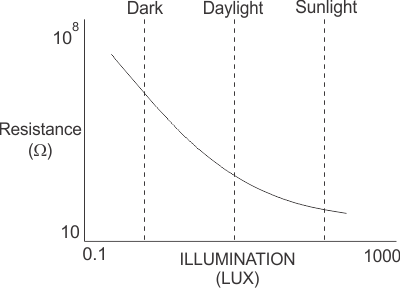
\includegraphics[width=8cm]{figuras/curva_ldr.png}
	\caption{Curva característica de resposta do LDR} \label{curva_ldr}
\end{figure}

